\chapter{Segmentation Paradigms and the First Baselines}\label{ch:paradigms}

\section{Introduction}\label{sec:paradigms-intro}
\epigraph{Essentially, all models are wrong, but some are useful.}{George Box and Norman Draper,
\emph{Empirical Model-Building and Response Surfaces} \citeyearpar[p.~424]{boxdraper1987}}

In this chapter we describe our first models. Before doing so, we need some vocabulary, because
computer vision distinguishes several kinds of segmentation, and the differences between them
turn out to be central to this problem. Section~\ref{sec:paradigms-kinds} defines semantic,
instance and panoptic segmentation. Sections~\ref{sec:paradigms-unet}--\ref{sec:paradigms-cc}
describe the simplest approach, in which a network labels each pixel as filament or background
and a separate rule then divides the filament pixels into objects. Section~\ref{sec:paradigms-results}
reports how well this approach worked, and Section~\ref{sec:paradigms-fragments} describes two
attempts to improve the rule that divides pixels into objects. Section~\ref{sec:paradigms-stop}
explains why we moved on to models that output objects directly, and
Section~\ref{sec:paradigms-decoders} surveys the three main families of such models.

\section{Semantic, instance and panoptic segmentation}\label{sec:paradigms-kinds}
Computer vision has three standard ways to say which pixels of an image belong to filaments. They
differ in what they say about \emph{identity}, that is, about which filament each pixel belongs to.

A \keyterm{semantic segmentation} assigns a class to every pixel. With a single class of interest,
it is a function from the image to a map of probabilities,
\begin{equation}
f_\theta : \R^{H\times W} \to [0,1]^{H\times W}, \qquad
f_\theta(\mathbf{x})_i = \Pr(\text{pixel } i \text{ is filament} \mid \mathbf{x}),
\label{eq:par-semantic}
\end{equation}
where $\mathbf{x}$ is the photograph and $\theta$ are the weights of the network. The map says
nothing about identity. Two filaments that touch become a single blob, and a single filament that
is interrupted by a faint stretch becomes two separate pieces.

An \keyterm{instance segmentation} returns a set of objects,
\begin{equation}
\{(m_k, s_k)\}_{k=1}^{K}, \qquad m_k \in \{0,1\}^{H\times W}, \quad s_k \in [0,1],
\label{eq:par-instance}
\end{equation}
consisting of a binary mask $m_k$ and a confidence score $s_k$ for each object. Identity is now
part of the answer. In general-purpose benchmarks such as COCO~\citep{coco}, the masks of two
instances are allowed to overlap.

A \keyterm{panoptic segmentation}~\citep{pq} gives every pixel exactly one owner, which is either
a ``stuff'' class, such as sky or road, or one particular instance of a ``thing'' class, such as a
car. Our competition is a panoptic problem with a single thing class: the background is the only
stuff, and each filament is a thing. The rule that no pixel may belong to two masks is the panoptic
constraint, and it is the reason why the metric is called Panoptic Quality.

\begin{figure}[t]
\centering
\begin{tikzpicture}[
  panel/.style={draw=inkmuted, line width=0.6pt, fill=gridline!45, minimum width=3.3cm,
                minimum height=2.45cm, rounded corners=2pt},
  fil/.style={line width=5.5pt, line cap=round, draw=#1}]
  \foreach \px/\name/\what in {0/semantic/{one map: is this\\ pixel a filament?},
                               3.9/instance/{one mask per object;\\ masks may overlap},
                               7.8/panoptic/{every pixel has\\ exactly one owner}}{
    \node[panel] at (\px,0) {};
    \node[title] at (\px,1.5) {\name};
    \node[note] at (\px,-1.62) {\what};
  }
  % semantic: one class; the two lower filaments touch and fuse
  \draw[fil=vizblue!75] (-1.25,0.62) .. controls (-0.6,0.95) and (0.2,0.3) .. (1.2,0.7);
  \draw[fil=vizblue!75] (-1.2,-0.35) .. controls (-0.7,-0.8) and (-0.1,-0.2) .. (0.45,-0.75);
  \draw[fil=vizblue!75] (0.2,-0.52) .. controls (0.55,-0.3) and (0.95,-0.45) .. (1.3,-0.1);
  % instance: one colour per object, translucent so the overlap shows
  \begin{scope}[xshift=3.9cm]
    \draw[fil=vizblue, draw opacity=0.7] (-1.25,0.62) .. controls (-0.6,0.95) and (0.2,0.3) .. (1.2,0.7);
    \draw[fil=vizorange, draw opacity=0.7] (-1.2,-0.35) .. controls (-0.7,-0.8) and (-0.1,-0.2) .. (0.45,-0.75);
    \draw[fil=vizaqua, draw opacity=0.7] (0.2,-0.52) .. controls (0.55,-0.3) and (0.95,-0.45) .. (1.3,-0.1);
    \draw[->, line width=0.5pt, draw=inkprimary] (0.75,-0.95) -- (0.3,-0.62);
    \node[note, anchor=west] at (0.62,-1.0) {overlap};
  \end{scope}
  % panoptic: opaque, lowest score painted first so the highest score owns contested pixels
  \begin{scope}[xshift=7.8cm]
    \draw[fil=vizaqua] (0.2,-0.52) .. controls (0.55,-0.3) and (0.95,-0.45) .. (1.3,-0.1);
    \draw[fil=vizorange] (-1.2,-0.35) .. controls (-0.7,-0.8) and (-0.1,-0.2) .. (0.45,-0.75);
    \draw[fil=vizblue] (-1.25,0.62) .. controls (-0.6,0.95) and (0.2,0.3) .. (1.2,0.7);
  \end{scope}
\end{tikzpicture}
\caption{The same three filaments as a semantic map, as instances and as a panoptic segmentation.
In the semantic map the two lower filaments touch and fuse into one blob. As instances they are
separate, but their masks overlap. The panoptic answer gives the contested pixels to one mask, here
the orange one, which has the higher score (Section~\ref{sec:masks-paint}).
\drawnin{book/chapters/ch06\_paradigms.tex}}
\label{fig:par-kinds}
\end{figure}

Figure~\ref{fig:par-kinds} shows the three kinds of answer for the same three filaments. To turn a
semantic answer into a panoptic one we must make two additional decisions: how to divide the
foreground pixels into objects, and who owns a pixel that two objects both claim. The second
decision is made by painting, which we described in Section~\ref{sec:masks-paint}. The rest of this
chapter is about the first decision, and about our first models, which made it after the network
had finished its work.

\section{An encoder--decoder for dense prediction}\label{sec:paradigms-unet}
Our first model (exp001) was a semantic segmentation model. This is the natural first attempt:
semantic segmentation is the most thoroughly studied problem in the field, and its output, a
probability for every pixel, is easy to inspect and to debug.

\subsection{The U-Net}\label{sec:par-unet-arch}
The \keyterm{U-Net}~\citep{unet}, a refinement of the fully convolutional network
of \citet{long2015}, is the standard architecture for dense prediction when the structures of
interest are small compared with the image. Figure~\ref{fig:par-unet} shows its
shape. The \keyterm{encoder} is an ordinary image classifier, such as a ResNet~\citep{resnet} or an
EfficientNet~\citep{efficientnet}, with its final classification layer removed. Each stage of the
encoder halves the height and width of its feature map and increases the number of channels. The
deep features therefore summarise a large part of the image, but they locate things only coarsely:
at the bottom of a typical encoder, one feature vector describes a block of $32\times32$ pixels.

The \keyterm{decoder} reverses the process. Each decoder stage doubles the resolution and then
\emph{concatenates} the encoder's feature map of the same size, carried across by a
\keyterm{skip connection}, before applying further convolutions. A final $1\times1$ convolution
produces one number $z_i$ for each pixel $i$, called a \keyterm{logit}, and the sigmoid function
turns it into a probability,
\begin{equation}
p_i = \sigmoid(z_i) = \frac{1}{1+e^{-z_i}}.
\end{equation}

The skip connections are what make this architecture suitable for filaments. The deep path of the
network can answer the question ``is there a filament somewhere around here?'' using a wide
context, while the skip connections answer the question ``which pixels, precisely?'' using features
computed before the resolution was reduced. A filament needs both answers. Its shape can extend
over hundreds of pixels, but its body is often only four or five pixels wide, and a structure that
narrow does not survive to the bottom of the encoder.

\begin{figure}[t]
\centering
\begin{tikzpicture}[
  fmap/.style={draw=#1!80!black, fill=#1!22, line width=0.5pt, inner sep=0pt},
  skipflow/.style={->, line width=0.7pt, draw=vizaqua!75!black, dashed},
  udflow/.style={->, line width=0.8pt, draw=inksecondary}]
  \node[inner sep=0pt] (in) at (-1.6,0) {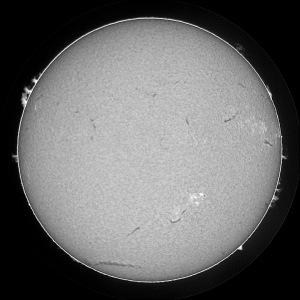
\includegraphics[width=1.25cm]{figures/thumb_input.png}};
  \node[note, below=2pt of in] {photograph};
  % encoder: resolution falls, channels grow
  \node[fmap=vizblue, minimum width=0.22cm, minimum height=1.8cm] (e0) at (0,0) {};
  \node[fmap=vizblue, minimum width=0.34cm, minimum height=1.2cm] (e1) at (0.9,-2.0) {};
  \node[fmap=vizblue, minimum width=0.50cm, minimum height=0.8cm] (e2) at (1.8,-3.6) {};
  \node[fmap=vizviolet, minimum width=0.72cm, minimum height=0.5cm] (b) at (3.7,-4.8) {};
  % decoder: resolution returns
  \node[fmap=vizorange, minimum width=0.50cm, minimum height=0.8cm] (d2) at (5.6,-3.6) {};
  \node[fmap=vizorange, minimum width=0.34cm, minimum height=1.2cm] (d1) at (6.5,-2.0) {};
  \node[fmap=vizorange, minimum width=0.22cm, minimum height=1.8cm] (d0) at (7.4,0) {};
  \node[box=vizorange, right=0.45cm of d0, text width=1.9cm] (out) {one logit per pixel\\ $p_i=\sigmoid(z_i)$};
  \draw[udflow] (in) -- (e0);
  \draw[udflow] (e0.south) -- node[note, left=2pt] {halve} (e1.north);
  \draw[udflow] (e1.south) -- node[note, left=2pt] {halve} (e2.north);
  \draw[udflow] (e2.south) |- (b.west);
  \draw[udflow] (b.east) -| (d2.south);
  \draw[udflow] (d2.north) -- node[note, right=2pt] {double} (d1.south);
  \draw[udflow] (d1.north) -- node[note, right=2pt] {double} (d0.south);
  \draw[udflow] (d0) -- (out);
  \draw[skipflow] (e0.east) -- node[note, above=1pt] {skip: copy and concatenate} (d0.west);
  \draw[skipflow] (e1.east) -- (d1.west);
  \draw[skipflow] (e2.east) -- (d2.west);
  \node[note, anchor=east] at (-0.25,-2.0) {1/2};
  \node[note, anchor=east] at (0.65,-3.6) {1/4};
  \node[note] at (3.7,-5.35) {bottleneck: 1/8 here, 1/32 in real encoders};
  \node[title, text=vizblue!80!black] at (0.2,1.25) {encoder};
  \node[title, text=vizorange!80!black] at (7.2,1.25) {decoder};
\end{tikzpicture}
\caption{A U-Net. The heights of the bars stand for spatial resolution and their widths for the
number of channels. The encoder halves the resolution at each stage; the decoder doubles it again
and concatenates the encoder's map of the same size (dashed skip connections). Real encoders use
five halvings, whereas the diagram shows three. \drawnin{book/chapters/ch06\_paradigms.tex}}
\label{fig:par-unet}
\end{figure}

\subsection{Our first model}\label{sec:par-exp001}
Experiment exp001 used \keyterm{U-Net++}~\citep{unetpp}, a variant of the U-Net in which each skip
connection passes through a small stack of nested convolution blocks, so that the encoder features
and the decoder features are more alike when they are joined. The encoder was an EfficientNet-B4
pretrained on ImageNet~\citep{deng2009}. The photographs are grey, whereas an ImageNet encoder
expects three colour channels, so we copied the grey image into all three. Each image was first
contrast-equalised with CLAHE~\citep{zuiderveld1994} (contrast-limited adaptive histogram
equalisation, with a clip limit of 2.0 on an $8\times8$
grid of tiles) and then blurred very slightly (a Gaussian with $\sigma=0.7$ pixels). The model was
trained on $512\times512$ inputs with batches of 8, a learning rate of $10^{-4}$ with a two-epoch
warm-up and a cosine decay~\citep{sgdr}, and mixed-precision arithmetic~\citep{mixedprecision} on
a T4 GPU. Early stopping ended
training at epoch 46; the best epoch was epoch 34.

\subsection{Example: the cost of resolution, measured before training}\label{sec:par-ceiling}
An input of $512\times512$ pixels is a quarter of the native width, so a filament four pixels wide
becomes one pixel wide. What is the best score that a model working at this resolution could
achieve? We answered this question before training anything, using a kind of measurement
that later became a habit (Section~\ref{sec:val-oracles}). We took the \emph{annotated} filament
masks and shrank their union to the training resolution, in the same way that the training targets
were built. We then thresholded the result, enlarged it back to $2048\times2048$ pixels, split it
into connected components (Section~\ref{sec:paradigms-cc}), and scored these components with PQ.
The result is the output of a \emph{perfect} semantic model at that resolution, so its score is an
upper bound on what the design can achieve:
\begin{center}\small
\begin{tabular}{@{}ccccc@{}}
\toprule
resolution & closing kernel & PQ & SQ & RQ \\
\midrule
512 & none & \textbf{0.7642} & 0.7660 & 0.9977 \\
512 & 5 px & 0.7589 & 0.7607 & 0.9977 \\
512 & 9 px & 0.7481 & 0.7508 & 0.9965 \\
1024 & none & \textbf{0.8692} & 0.8702 & 0.9988 \\
1024 & 5 px & 0.8430 & 0.8449 & 0.9977 \\
\bottomrule
\end{tabular}
\end{center}

We drew three conclusions from this table, and each of them changed a decision. First, connected
components recover the filaments almost perfectly from a perfect mask (RQ is 0.998), so separating
the filaments from each other is not difficult \emph{when the mask is correct}. Second, all of the
loss is in SQ: shrinking the image blurs every boundary, which costs about a quarter of the IoU at
512 pixels and about an eighth at 1024. Third, morphological \emph{closing}~\citep{serra1982} (a dilation followed
by an erosion, which rejoins nearby fragments) makes matters worse, because it widens every mask by
more than the rejoined fragments are worth. We therefore switched closing off.

\section{Losses for imbalanced segmentation}\label{sec:par-loss}
Filament pixels make up about one percent of the pixels on the disk. This \keyterm{class
imbalance} causes problems for the standard loss function. Plain binary cross-entropy is already
99\% ``correct'' for a network that predicts background everywhere, so it gives weak and misleading
gradients early in training. In exp001 we combined two standard remedies.

The first is a \keyterm{weighted binary cross-entropy}, which makes a missed filament pixel $w$
times as costly as a false one:
\begin{equation}
\mathcal{L}_{\mathrm{BCE}} = -\frac{1}{N}\sum_{i=1}^{N}\Big[\,w\,y_i\log p_i + (1-y_i)\log(1-p_i)\Big],
\qquad w = 8,
\label{eq:par-bce}
\end{equation}
where $y_i\in\{0,1\}$ is the target for pixel $i$ and $N$ is the number of pixels.

The second is the \keyterm{soft Dice loss}~\citep{vnet}, which replaces the counts in the Dice coefficient of
Section~\ref{sec:masks-iou} with probabilities, so that it can be differentiated:
\begin{equation}
\mathcal{L}_{\mathrm{Dice}} = 1 - \frac{2\sum_i p_i y_i + \epsilon}{\sum_i p_i + \sum_i y_i + \epsilon},
\qquad \epsilon = 1.
\label{eq:par-dice}
\end{equation}
The Dice coefficient measures overlap relative to the size of the objects, so the very large number
of easy background pixels cannot dominate it~\citep{sudre2017}. We can see this by computing its gradient. Write
$I=\sum_i p_i y_i$ for the soft intersection and $S=\sum_i p_i+\sum_i y_i+\epsilon$. Then
\begin{equation}
\frac{\partial\mathcal{L}_{\mathrm{Dice}}}{\partial p_i} = \frac{(2I+\epsilon) - 2y_iS}{S^2}.
\end{equation}
For a background pixel ($y_i=0$) the gradient is positive, so gradient descent lowers $p_i$. For a
filament pixel ($y_i=1$) it is negative, since $I$ can exceed neither $\sum_i p_i$ nor $\sum_i y_i$,
so that $2I+\epsilon\le S<2S$; gradient descent therefore raises $p_i$. The quantities $I$ and
$S$ measure the soft predicted foreground and the annotated foreground, and neither of them grows
with the number of correctly classified background pixels, so the gradients do not shrink when the
objects occupy only a small part of the image. The smoothing
constant $\epsilon$ prevents the expression $0/0$ on an image that contains no filament. The total
loss was the average of the two terms, $\mathcal{L}=\tfrac12\mathcal{L}_{\mathrm{BCE}}+\tfrac12
\mathcal{L}_{\mathrm{Dice}}$, as Listing~\ref{lst:par-loss} shows.

\begin{lstlisting}[caption={Weighted cross-entropy plus soft Dice. Condensed from
\file{experiments/exp\_001\_baseline/src/model.py}.},label=lst:par-loss]
class CombinedLoss(nn.Module):
    def __init__(self, bce_weight=0.5, dice_weight=0.5, pos_weight=8.0):
        super().__init__()
        self.bce_weight, self.dice_weight = bce_weight, dice_weight
        self.bce = nn.BCEWithLogitsLoss(pos_weight=torch.tensor(pos_weight))

    def forward(self, logits, targets):            # both (batch, 1, H, W)
        bce = self.bce(logits, targets)
        probs = torch.sigmoid(logits)
        intersection = (probs * targets).sum((2, 3))
        cardinality = probs.sum((2, 3)) + targets.sum((2, 3))
        # +1 keeps an image with no filament from giving 0/0
        dice = 1.0 - ((2.0 * intersection + 1.0) / (cardinality + 1.0)).mean()
        return self.bce_weight * bce + self.dice_weight * dice
\end{lstlisting}

\section{From probabilities to instances}\label{sec:paradigms-cc}
A probability map is not yet a submission. In exp001 we turned it into instances with the simplest
possible rule, summarised in Algorithm~\ref{alg:par-cc}.

\begin{algorithmblock}{From a probability map to disjoint instances (exp001)\label{alg:par-cc}}
\item \textbf{input:} a $512\times512$ probability map $P$; threshold $\tau=0.5$; minimum area $a_{\min}=150$
\item enlarge $P$ to $2048\times2048$ by bilinear interpolation;
\item $B\leftarrow[\,P\ge\tau\,]$, a binary mask;
\item (optionally) close small gaps in $B$; this step was switched off;
\item remove every pixel of $B$ that lies outside the solar disk;
\item label the 8-connected components of $B$;
\item \textbf{return} the components whose area is at least $a_{\min}$, largest first
\end{algorithmblock}

Two details deserve comment. The map is enlarged \emph{before} it is thresholded, because enlarging
a thresholded map would turn every smooth edge into a staircase. The minimum area of 150 pixels
removes specks; the smallest one percent of annotated filaments cover about 208 pixels, so very few
real filaments are that small.

Two foreground pixels belong to the same \keyterm{connected component} if they can be joined by a
path of foreground pixels~\citep{rosenfeld1966}. With \keyterm{8-connectivity}, each step of such a path may go to any of
the eight neighbouring pixels, including the diagonal ones; with 4-connectivity, only to the four
that share an edge. Figure~\ref{fig:par-cc} works through a small example. Since the connected
components partition the foreground, the resulting masks are automatically disjoint, and no
painting step is needed.

\begin{figure}[t]
\centering
\begin{tikzpicture}[pcell/.style={minimum size=0.27cm, inner sep=0pt, draw=white, line width=0.4pt}]
  % panel 1: probabilities in tenths
  \foreach \row [count=\y from 0] in {{0,1,1,0,0,0,0,0,0,0},{1,7,8,6,2,0,0,0,1,0},
      {0,2,6,8,4,7,8,1,0,0},{0,0,1,2,1,2,9,8,2,0},{0,0,0,0,0,1,7,9,6,1},{0,0,0,0,0,0,1,2,1,0}}{
    \foreach \p [count=\x from 0] in \row {
      \pgfmathtruncatemacro{\shade}{\p*10}
      \node[pcell, fill=vizblue!\shade!white] at (\x*0.27, -\y*0.27)
        {\tiny\sffamily\ifnum\p>6 \color{white}\else\color{inksecondary}\fi\p};
    }
  }
  % panel 2: threshold at 0.5
  \begin{scope}[xshift=3.7cm]
  \foreach \row [count=\y from 0] in {{0,1,1,0,0,0,0,0,0,0},{1,7,8,6,2,0,0,0,1,0},
      {0,2,6,8,4,7,8,1,0,0},{0,0,1,2,1,2,9,8,2,0},{0,0,0,0,0,1,7,9,6,1},{0,0,0,0,0,0,1,2,1,0}}{
    \foreach \p [count=\x from 0] in \row {
      \ifnum\p>4 \node[pcell, fill=inkprimary!75] at (\x*0.27, -\y*0.27) {};
      \else \node[pcell, fill=gridline!60] at (\x*0.27, -\y*0.27) {}; \fi
    }
  }
  \end{scope}
  % panel 3: component labels
  \begin{scope}[xshift=7.4cm]
  \foreach \row [count=\y from 0] in {{0,0,0,0,0,0,0,0,0,0},{0,1,1,1,0,0,0,0,0,0},
      {0,0,1,1,0,2,2,0,0,0},{0,0,0,0,0,0,2,2,0,0},{0,0,0,0,0,0,2,2,2,0},{0,0,0,0,0,0,0,0,0,0}}{
    \foreach \cl [count=\x from 0] in \row {
      \ifcase\cl \node[pcell, fill=gridline!60] at (\x*0.27, -\y*0.27) {};
      \or \node[pcell, fill=vizblue] at (\x*0.27, -\y*0.27) {};
      \or \node[pcell, fill=vizorange] at (\x*0.27, -\y*0.27) {}; \fi
    }
  }
  \end{scope}
  \node[title] at (1.215,0.45) {probability, in tenths};
  \node[title] at (4.915,0.45) {threshold at 0.5};
  \node[title] at (8.615,0.45) {8-connected components};
  \draw[flow] (2.75,-0.675) -- (3.55,-0.675);
  \draw[flow] (6.45,-0.675) -- (7.25,-0.675);
  \draw[vizorange, line width=1.1pt] (0.945,-0.675) rectangle (1.215,-0.405);
  \node[note] at (1.215,-1.8) {outlined: 0.4, just below the threshold};
\end{tikzpicture}
\caption{Connected-component labelling of a small probability map. One faint pixel (0.4) lies
below the threshold, so what may be a single filament becomes two components, shown in blue and
orange. If both halves belong to one annotated filament, each covers only part of it; if neither
half reaches an IoU of 0.5 with the filament, PQ counts two false positives and one false negative.
\drawnin{book/chapters/ch06\_paradigms.tex}}
\label{fig:par-cc}
\end{figure}

Listing~\ref{lst:par-cc} gives the implementation, using OpenCV's connected-component labelling.

\begin{lstlisting}[caption={Semantic probabilities to disjoint instances. Condensed from
\file{experiments/exp\_001\_baseline/src/postprocess.py}.},label=lst:par-cc]
def probability_to_instances(probability, threshold, min_area, closing_kernel, disk=None):
    # 1. enlarge to the native frame BEFORE thresholding, or every edge becomes a staircase
    upsampled = cv2.resize(probability.astype(np.float32), (2048, 2048),
                           interpolation=cv2.INTER_LINEAR)
    binary = (upsampled >= threshold).astype(np.uint8)            # 2. threshold
    if closing_kernel > 1:                                         # 3. optional closing
        kernel = cv2.getStructuringElement(cv2.MORPH_ELLIPSE, (closing_kernel, closing_kernel))
        binary = cv2.morphologyEx(binary, cv2.MORPH_CLOSE, kernel)
    if disk is not None:                                           # 4. nothing off the disk
        binary &= disk.mask(binary.shape)
    n, labels, stats, _ = cv2.connectedComponentsWithStats(binary, connectivity=8)
    instances = [(stats[k, cv2.CC_STAT_AREA], (labels == k).astype(np.uint8))
                 for k in range(1, n) if stats[k, cv2.CC_STAT_AREA] >= min_area]
    instances.sort(key=lambda item: -item[0])                      # 5. largest first
    return [mask for _, mask in instances]
\end{lstlisting}

\section{Results of the dense models}\label{sec:paradigms-results}
Our first model, exp001, scored a PQ of 0.2957 on the 180 validation records and 0.26 on the public
leaderboard. The components of its score are more informative than the total:
\begin{center}\small
\setlength{\tabcolsep}{4pt}
\begin{tabular}{@{}lccccc@{}}
\toprule
model & PQ & SQ & RQ & TP / FP / FN & instances per image \\
\midrule
exp001 (U-Net++, 512) & 0.2957 & 0.629 & 0.470 & 673 / 866 / 652 & 8.6 (annotations: 7.4) \\
\bottomrule
\end{tabular}
\end{center}
The matched masks were reasonable, with a mean IoU of 0.63, but recognition was poor. Fewer than
half of the predictions, and only about half of the annotated filaments, found a partner. The model
was not failing wholesale: only 4 of the 180 records scored zero, so it was doing something useful
on almost every photograph.

Our second dense model, exp004, removed the two most obvious limitations of the first. It trained a
U-Net with a ResNet-34 encoder at twice the resolution, $1024\times1024$, for 300 epochs, until the
validation loss had stopped improving for many epochs. It ran on the eight cores of a Kaggle TPU in
3.8 hours (Appendix~\ref{app:infra}), and at test time it averaged the probability maps predicted
for flipped copies of the image. It scored 0.28 on the public leaderboard, an improvement of only
two hundredths for four times as many pixels and a fully converged model. It also emitted 9.50
instances per image, against 7.4 in the annotations.

\section{Grouping pixels by other means}\label{sec:paradigms-fragments}
Our first explanation for the poor recognition of exp001 was \keyterm{fragmentation}. A filament
that the seeing conditions break into several dark patches is a single object to the annotator, but
connected components cannot know that, so they return one instance per patch, as in
Figure~\ref{fig:par-cc}. Each patch covers only part of the filament, so none of them reaches an IoU
of 0.5, and one physical error becomes one false negative plus several false positives. This
explanation is plausible, and it makes a testable prediction: the model should emit many more
instances than there are filaments.

It turned out that it did not. The model emitted 8.6 instances per image against 7.4 in the
annotations, a ratio of 1.16, which indicates at most a mild over-segmentation.
 We had promoted the explanation to a finding without testing it. Before we noticed
this, we had designed two decoders to fix the supposed problem. We describe them next, together
with the tests that we used to evaluate them.

\subsection{Seeding instances on spines}\label{sec:par-spine}
Every one of the \AllFilaments{} annotations includes a spine, a polyline along the filament's axis
(Section~\ref{sec:data-spines}). Our plan for exp004 was to exploit this. Even when a filament is
broken into patches, it has a single spine. We would therefore predict the spine as a second output
channel of the network, treat each connected piece of the predicted spine as one filament, and give
every pixel of the mask to its nearest spine. This assignment is a \keyterm{Voronoi partition} of
the mask, and it can be computed in a single pass by a distance transform that also reports
\emph{which} seed pixel is nearest to each pixel. Listing~\ref{lst:par-spine} shows the
implementation.

\begin{lstlisting}[caption={Spine-seeded instances. Condensed from
\file{experiments/exp\_004\_spine\_tpu/src/decompose.py}.},label=lst:par-spine]
def decompose(mask, spine, min_area=150, min_spine_area=8):
    spine = ((spine > 0) & (mask > 0)).astype(np.uint8)        # spines inside the mask only
    n, spine_labels, stats, _ = cv2.connectedComponentsWithStats(spine, connectivity=8)
    keep = [k for k in range(1, n) if stats[k, cv2.CC_STAT_AREA] >= min_spine_area]
    if not keep:
        return connected_components(mask, min_area)            # fall back to exp001
    seeds = np.zeros_like(spine_labels, dtype=np.int32)
    for new, old in enumerate(keep, start=1):
        seeds[spine_labels == old] = new
    # For every non-seed pixel: the index of its nearest seed pixel (straight-line distance).
    _, index = cv2.distanceTransformWithLabels((seeds == 0).astype(np.uint8), cv2.DIST_L2, 3,
                                               labelType=cv2.DIST_LABEL_PIXEL)
    lookup = np.concatenate([[0], seeds.reshape(-1)[np.flatnonzero(seeds)]])
    assigned = np.where(mask > 0, lookup[index], 0)             # seed index -> spine label
    return [m for m in ((assigned == k).astype(np.uint8) for k in range(1, len(keep) + 1))
            if m.sum() >= min_area]
\end{lstlisting}

\begin{figure}[t]
\centering
\begin{tikzpicture}[
  piece/.style={line width=6pt, line cap=round, draw=#1},
  spn/.style={line width=0.8pt, draw=inkprimary, dash pattern=on 2.2pt off 1.4pt}]
  \foreach \sx/\lab in {0/{(a) mask and predicted spines}, 3.9/{(b) connected components: one}, 7.8/{(c) spine seeding: two}}{
    \node[note] at (\sx+1.3,-1.25) {\lab};
  }
  % (a) the union mask in grey with both spines
  \draw[piece=inkmuted!55] (0,0) .. controls (0.6,0.45) and (1.2,0.45) .. (1.7,0.05);
  \draw[piece=inkmuted!55] (1.45,0.2) .. controls (1.8,-0.2) and (2.2,-0.6) .. (2.65,-0.75);
  \draw[spn] (0,0) .. controls (0.6,0.45) and (1.2,0.45) .. (1.7,0.05);
  \draw[spn] (1.45,0.2) .. controls (1.8,-0.2) and (2.2,-0.6) .. (2.65,-0.75);
  % (b) connected components: the touching filaments form one component
  \begin{scope}[xshift=3.9cm]
    \draw[piece=vizblue] (0,0) .. controls (0.6,0.45) and (1.2,0.45) .. (1.7,0.05);
    \draw[piece=vizblue] (1.45,0.2) .. controls (1.8,-0.2) and (2.2,-0.6) .. (2.65,-0.75);
  \end{scope}
  % (c) spine seeding: each pixel goes to its nearest spine
  \begin{scope}[xshift=7.8cm]
    \draw[piece=vizorange] (1.45,0.2) .. controls (1.8,-0.2) and (2.2,-0.6) .. (2.65,-0.75);
    \draw[piece=vizblue] (0,0) .. controls (0.6,0.45) and (1.2,0.45) .. (1.7,0.05);
  \end{scope}
\end{tikzpicture}
\caption{What spine seeding can do. Two filaments touch, so their union forms one connected
component (b). Their spines are separate, so assigning each pixel to its nearest spine divides the
mask into two instances (c). Rejoining the patches of a broken filament is harder, because the
spine is first cut to the mask, so a gap that severs the mask also severs its spine.
\drawnin{book/chapters/ch06\_paradigms.tex}}
\label{fig:par-spine}
\end{figure}

The first line of Listing~\ref{lst:par-spine} contains a detail that the design description did
not mention. It intersects the spine with the mask, so a gap that cuts the mask in two also cuts the
spine in two, and each patch keeps its own seed. A patch is rejoined to its neighbour only when it
contains fewer than 8 spine pixels of its own. The method therefore \emph{separates} two touching
filaments with distinct spines reliably (Figure~\ref{fig:par-spine}), but it rejoins the pieces of
a broken filament only occasionally.

Before we spent any TPU time on the idea, we tested it without training a model. The test took the
annotated masks, imitated fragmentation by eroding them and then dilating them with a $k\times k$
square (which severs thin necks), and scored both decoders against the true instances on 60
validation records:
\begin{center}\small
\begin{tabular}{@{}ccccc@{}}
\toprule
erosion $k$ & predicted / true instances & components PQ & spine PQ & difference \\
\midrule
0 & 1.00 & 1.0000 & 1.0000 & $+0.0000$ \\
3 & 0.99 & 0.8947 & 0.8952 & $+0.0005$ \\
5 & 0.80 & 0.5059 & 0.5058 & $-0.0001$ \\
7 & 0.66 & 0.2875 & 0.2874 & $-0.0001$ \\
\bottomrule
\end{tabular}
\end{center}
Spine seeding gained nothing, and we trained exp004 without a spine output. The second column shows
why the test could not have shown a gain even if one existed: under erosion the number of instances
\emph{fell}. The degradation deleted small filaments instead of splitting large ones, so it never
produced the fragmentation that it was meant to imitate.

\subsection{Voting for centres}\label{sec:par-offset}
The second decoder was taken from Panoptic-DeepLab~\citep{panopticdeeplab}. Instead of asking
whether pixels touch, it asks each pixel where the centre of its object lies. For an instance $k$
with pixel set $S_k$, let its centre be the centroid $\mathbf{c}_k = |S_k|^{-1}\sum_{\mathbf{p}\in
S_k}\mathbf{p}$. The network predicts two dense maps. The first is a heat map whose target is a
Gaussian bump at each centre,
\begin{equation}
h(\mathbf{q}) = \max_k \exp\!\left(-\frac{\lVert\mathbf{q}-\mathbf{c}_k\rVert^2}{2\sigma^2}\right),
\qquad \sigma = 8 \text{ px}.
\end{equation}
The second is an \keyterm{offset field}, whose target at each filament pixel is the vector from the
pixel to the centre of its own filament, $\mathbf{o}(\mathbf{p}) = \mathbf{c}_k - \mathbf{p}$ for
$\mathbf{p}\in S_k$. At test time, the centres $\hat{\mathbf{c}}_1,\dots,\hat{\mathbf{c}}_M$ are the
local maxima of the predicted heat map that exceed 0.3 within a $21\times21$ window, and each
foreground pixel joins the centre nearest to the point it votes for:
\begin{equation}
\hat k(\mathbf{p}) = \argmin_{m}\,\big\lVert\, \mathbf{p} + \hat{\mathbf{o}}(\mathbf{p}) - \hat{\mathbf{c}}_m \big\rVert .
\label{eq:par-vote}
\end{equation}
Two disconnected patches of one filament point to the same centre, so they are joined, and two
touching filaments point to different centres, so they are separated. Connected components can do
neither.

\begin{figure}[t]
\centering
\begin{tikzpicture}[
  fl/.style={line width=7pt, line cap=round, draw=#1, draw opacity=0.28},
  px/.style={circle, fill=#1, inner sep=0pt, minimum size=4pt},
  vote/.style={->, line width=0.55pt, draw=#1, >={Stealth[length=1.4mm]}},
  ctr/.style={draw=#1, line width=1.1pt, cross out, minimum size=5pt, inner sep=0pt}]
  \foreach \sx in {0,5.6}{
    \begin{scope}[xshift=\sx cm]
      \draw[fl=vizblue] (0,0.92) .. controls (0.7,1.25) and (1.6,1.3) .. (2.4,1.02);
      \draw[fl=vizorange] (0.2,-0.02) .. controls (0.8,0.12) and (1.6,0.25) .. (2.3,0.3);
      \node[ctr=vizblue!80!black] at (1.2,1.12) {};
      \node[ctr=vizorange!80!black] at (1.28,0.17) {};
    \end{scope}
  }
  % (a) exact offsets: every vote lands on its own centre
  \foreach \x/\y in {0.1/0.95, 0.6/1.12, 1.8/1.2, 2.3/1.05}
    { \node[px=vizblue] (p) at (\x,\y) {}; \draw[vote=vizblue] (p) -- (1.2,1.12); }
  \foreach \x/\y in {0.3/0.0, 0.8/0.1, 1.8/0.24, 2.2/0.29}
    { \node[px=vizorange] (p) at (\x,\y) {}; \draw[vote=vizorange] (p) -- (1.28,0.17); }
  % (b) noisy offsets: one orange pixel's vote lands nearer the blue centre
  \begin{scope}[xshift=5.6cm]
    \foreach \x/\y/\tx/\ty in {0.1/0.95/1.35/1.0, 0.6/1.12/1.0/1.27, 1.8/1.2/1.1/0.97, 2.3/1.05/1.45/1.22}
      { \node[px=vizblue] (p) at (\x,\y) {}; \draw[vote=vizblue] (p) -- (\tx,\ty); }
    \foreach \x/\y/\tx/\ty in {0.3/0.0/1.1/0.3, 2.2/0.29/1.0/0.08, 1.8/0.24/1.45/0.02}
      { \node[px=vizorange] (p) at (\x,\y) {}; \draw[vote=vizorange] (p) -- (\tx,\ty); }
    \node[px=vizblue, draw=inkprimary, line width=0.6pt, minimum size=5pt] (bad) at (0.8,0.1) {};
    \draw[vote=inkprimary] (bad) -- (1.15,0.78);
    \node[note, anchor=west] at (2.55,0.62) {vote lands nearer the\\ blue centre: pixel\\ joins the wrong filament};
  \end{scope}
  \node[note] at (1.2,-0.62) {(a) exact offsets};
  \node[note] at (6.8,-0.62) {(b) offsets with noise};
\end{tikzpicture}
\caption{Centre voting. Each filament pixel (dot) predicts a vector to the centre of its filament
(cross), and joins the detected centre nearest to where its vector lands
(Equation~\eqref{eq:par-vote}). When the offsets are noisy (b), a vote from the orange filament
lands closer to the blue centre, and that pixel is assigned to the wrong filament.
\drawnin{book/chapters/ch06\_paradigms.tex}}
\label{fig:par-offset}
\end{figure}

We tested this decoder in the same way, again starting from the annotated masks with exact targets,
and then adding Gaussian noise of several sizes to the offsets to imitate an imperfect
network (50 validation records):
\begin{center}\small
\begin{tabular}{@{}cccccc@{}}
\toprule
 & \multicolumn{2}{c}{connected components} & \multicolumn{2}{c}{centre voting} & \\
\cmidrule(lr){2-3}\cmidrule(lr){4-5}
offset noise (px) & PQ & RQ & PQ & RQ & difference in PQ \\
\midrule
0 & 0.9995 & 1.000 & 1.0000 & 1.000 & $+0.0005$ \\
5 & 0.9995 & 1.000 & 0.9938 & 0.997 & $-0.0057$ \\
15 & 0.9995 & 1.000 & 0.9694 & 0.989 & $-0.0301$ \\
30 & 0.9995 & 1.000 & 0.8336 & 0.932 & $-0.1658$ \\
\bottomrule
\end{tabular}
\end{center}
The grouping degrades steeply once the offsets are wrong by a realistic margin
(Figure~\ref{fig:par-offset}), and the offsets predicted by a trained network are wrong by a
realistic margin.

\subsection{Ablations need headroom}\label{sec:par-headroom}
Both of these tests started from the annotated masks, and on annotated masks plain connected
components already score 0.9995. No decoder could beat that by more than 0.0005, so the tests
could reveal a decoder's losses but never its gains. The general lesson is that before running an
ablation we should compute what the control scores under the same conditions. If the control is
already at the ceiling, the ablation cannot answer the question it was designed for. In this case,
only \emph{predicted} masks could have settled the question, and predicted masks require a training
run.

\section{Why we abandoned the dense approach}\label{sec:paradigms-stop}
By this time we had trained our first instance segmentation model, which is the subject of the next
chapter, and could compare the approaches directly:
\begin{center}\small
\setlength{\tabcolsep}{4pt}
\begin{tabular}{@{}llccc@{}}
\toprule
run & model, input size & epochs & SQ / RQ & public \\
\midrule
exp001 & dense U-Net++, 512 & 46 & 0.629 / 0.470 & 0.26 \\
exp004 & dense U-Net, 1024 & 300 (converged) & -- & 0.28 \\
exp002 & YOLO11m instances, 1280 & 149 (stopped early) & 0.643 / 0.581 & 0.32 \\
\bottomrule
\end{tabular}
\end{center}
Doubling the resolution and training to convergence gained two hundredths. An instance model that
had been stopped while it was still improving beat both dense models by four hundredths or more.
Its matched masks were only slightly better (SQ 0.643 against 0.629); its gain came from recognition
(RQ 0.581 against 0.470, an improvement of about a quarter). We concluded that the limiting factor
was the paradigm itself, rather than the training budget or the resolution, and we moved on to
models that output instances directly.

We did not prove this conclusion. We never isolated the
mechanism that held the dense models back: fragmentation had been ruled out as the main cause, and
the decoder tests could not have detected it anyway. What the evidence does show is narrower. We
removed the two limitations that were easy to remove, and the score hardly moved.

The dense approach did not disappear from the project altogether. Much later, in exp085, we trained
a new semantic model based on a recent paper on solar filaments by
\citet{hu2026morden}.\footnote{The paper calls its model MORDEN. Our network adapts the
architecture of the authors' public code (released under the MIT licence), reduced in size to fit a
16 GB T4 GPU and given a second output for the spine.} It used $5\times5$ convolutions, instance
normalisation~\citep{ulyanov2016}, several parallel
branches at different scales, and three input channels (the raw image, a CLAHE version and a map of
local dark contrast). On its own it scored a PQ of only 0.3227, far below the instance models, but
its probability maps turned out to be useful as \emph{evidence} for deciding which of an instance
model's doubtful masks to keep (Section~\ref{sec:recall-semantic}).

\section{Three ways to output instances}\label{sec:paradigms-decoders}
Models that output instances directly differ mainly in \emph{when} they decide identity.
Figure~\ref{fig:par-families} sets the three main families side by side, and we met all three
during the project.

\begin{figure}[t]
\centering
\begin{tikzpicture}[
  lane/.style={box=#1, text width=1.85cm, minimum height=1.05cm, font=\sffamily\scriptsize,
               execute at begin node={\hyphenpenalty=10000}}]
  \foreach \y/\ttl in {0/{two-stage: detect boxes, then a mask per box (Mask R-CNN)},
                        -2.1/{one-stage with prototypes (YOLACT, YOLO segmentation)},
                        -4.2/{query-based set prediction (DETR, MaskFormer, Mask2Former)}}{
    \node[title, anchor=west] at (-1.07,\y+0.92) {\ttl};
  }
  \node[lane=inkmuted] (a1) at (0,0) {photograph};
  \node[lane=inkmuted] (a2) at (2.55,0) {backbone features};
  \node[lane=inkmuted] (a3) at (5.1,0) {box proposals};
  \node[lane=inkmuted] (a4) at (7.65,0) {crop a fixed-size feature per box};
  \node[lane=inkmuted] (a5) at (10.2,0) {small mask per box, pasted into it};
  \node[lane=vizblue] (b1) at (0,-2.1) {photograph};
  \node[lane=vizblue] (b2) at (2.55,-2.1) {backbone features};
  \node[lane=vizblue] (b3) at (5.1,-2.1) {$k$ prototype masks for the whole image};
  \node[lane=vizblue] (b4) at (7.65,-2.1) {per detection: a box and $k$ coefficients};
  \node[lane=vizblue] (b5) at (10.2,-2.1) {mask $=\sigmoid(\sum_j c_jP_j)$ inside the box};
  \node[lane=vizorange] (c1) at (0,-4.2) {photograph};
  \node[lane=vizorange] (c2) at (2.55,-4.2) {per-pixel embeddings};
  \node[lane=vizorange] (c3) at (5.1,-4.2) {$N$ learned queries attend to the image};
  \node[lane=vizorange] (c4) at (7.65,-4.2) {per query: class score, mask embedding};
  \node[lane=vizorange] (c5) at (10.2,-4.2) {mask $=\sigmoid(\mathbf{e}_q^{\top}\mathbf{F})$, one per query};
  \foreach \lane in {a,b,c}{
    \draw[flow] (\lane1) -- (\lane2); \draw[flow] (\lane2) -- (\lane3);
    \draw[flow] (\lane3) -- (\lane4); \draw[flow] (\lane4) -- (\lane5);
  }
\end{tikzpicture}
\caption{Three families of instance segmentation models. Two-stage models decide identity by
proposing boxes. Prototype models predict a shared set of mask shapes once per image and mix them
differently for each detection. Query-based models learn a fixed set of object slots and are trained
to use each slot for at most one object. \drawnin{book/chapters/ch06\_paradigms.tex}}
\label{fig:par-families}
\end{figure}

\paragraph{Two-stage models.} Mask R-CNN~\citep{maskrcnn}, which extends the Faster R-CNN
detector~\citep{ren2015}, first proposes boxes that may contain objects. It then crops a fixed-size feature map from inside each box and predicts a small mask for
it, typically $28\times28$ cells, which is stretched to fill the box. We met this family through a
public notebook that combined Mask R-CNN with a U-Net that refined each crop. In exp043 and exp044
we reproduced the notebook byte for byte and found that its advertised score was out of date: its
live public score was 0.34. We did not pursue this family further.

\paragraph{One-stage models with prototypes.} YOLACT~\citep{yolact} and the YOLO segmentation
models~\citep{yolo,ultralytics} predict, once per image, a small set of $k$ \keyterm{prototype}
masks $P_1,\dots,P_k$ that cover the whole image, and for each detected box a vector of $k$
coefficients $c_1,\dots,c_k$. The mask of a detection is the sigmoid of the weighted sum of the
prototypes, cropped to its box. Identity comes from the detector, and shape comes from mixing the
shared prototypes. This family carried our public score from 0.32 to 0.39, and
Chapters~\ref{ch:yolo}--\ref{ch:recall} are about it.

\paragraph{Query-based set prediction.} DETR~\citep{detr} and its segmentation descendants,
MaskFormer~\citep{maskformer} and Mask2Former~\citep{mask2former}, learn a fixed number $N$ of
\keyterm{queries}. Each query is a learned vector that looks at the image through attention and
then outputs a class score and an embedding vector $\mathbf{e}_q$. The query's mask is the sigmoid
of the dot product between $\mathbf{e}_q$ and the per-pixel embedding $\mathbf{F}$ at every pixel.
During training, a one-to-one matching pairs each annotated object with exactly one query, so the
model learns to describe each object once. This family produced our best model, and
Chapters~\ref{ch:transformers}--\ref{ch:submission} explain it in detail.

\section*{Exercises}
\begin{exercise}{Connected components by hand}
Relabel the middle panel of Figure~\ref{fig:par-cc} using 4-connectivity. Does the number of
components change? Then lower the threshold to 0.4 and label the map again. What happens, and what
would the change cost if the two pieces were in fact two separate filaments?
\end{exercise}

\begin{exercise}{The Dice gradient}
Derive the gradient of Equation~\eqref{eq:par-dice} with respect to $p_i$, and show that it is
always negative for a filament pixel, whatever the other predictions are. Then compute the gradient
of the unweighted cross-entropy for the same pixel, and compare how the two gradients depend on the
number of background pixels.
\end{exercise}

\begin{exercise}{A design ceiling}
Run \file{experiments/exp\_001\_baseline/src/ceiling\_analysis.py}, which needs only the annotation
file. Add a row for a resolution of 2048 (no shrinking at all), and explain why its PQ is not
exactly 1. (Hint: look at how the targets are thresholded.)
\end{exercise}

\begin{exercise}{Why the ablation shrank the instances}
In the spine ablation, an erosion followed by a dilation with a $7\times7$ square reduced the number
of instances to 0.66 of the true number. Using the filament widths described in
Section~\ref{sec:data-sizes}, explain which filaments disappear, and why none of them are split.
\end{exercise}

\begin{exercise}{How wrong can the offsets be?}
For every validation record, compute the centroid of each annotated filament and the distance from
each centroid to the nearest centroid of another filament in the same record, and plot the
distribution of these distances. At what offset error does Equation~\eqref{eq:par-vote} start to
assign pixels to the wrong filament in a typical record? Does your answer agree with the ablation
table of Section~\ref{sec:par-offset}?
\end{exercise}
